\documentclass[12pt,letterpaper]{exam}
\usepackage[lmargin=1in,rmargin=1in,tmargin=1in,bmargin=1in]{geometry}
\usepackage{../style/exams}

% -------------------
% Course & Exam Information
% -------------------
\newcommand{\course}{MAT 108: Exam 3}
\renewcommand{\term}{Fall -- 2023}
\newcommand{\examdate}{12/14/2023}
\newcommand{\timelimit}{85 Minutes}

\setbool{hideans}{true} % Student: True; Instructor: False

% -------------------
% Content
% -------------------
\begin{document}

\examtitle
\instructions{Write your name on the appropriate line on the exam cover sheet. This exam contains \numpages\ pages (including this cover page) and \numquestions\ questions. Check that you have every page of the exam. Answer the questions in the spaces provided on the question sheets. Be sure to answer every part of each question and show all your work. If you run out of room for an answer, continue on the back of the page --- being sure to indicate the problem number.} 
\scores
\bottomline
\newpage

% ---------
% Questions
% ---------
\begin{questions}

% Question 1
\newpage
\question[10] Find the dual problem for the linear programming problem below. 
	\[
	\begin{gathered}
	\min w= 3y_1 - y_2 + 7y_3  \\
	\begin{cases}
	y_1 + y_2 + y_3 \geq 4 \\
	11y_1 + 15y_3 \geq 15 \\
	3y_1 + y_2 - y_3 \geq -9 \\
	8y_1 - 6y_2 + y_3 \leq 19 \\
	y_1, y_2, y_3 \geq 0
	\end{cases}
	\end{gathered}
	\] \pspace

First, we need every inequality to be of the form `$\geq$' a number. We multiply both sides of the fourth inequality by $-1$ to place this inequality in this form. This gives us the following inequalities (ignoring the non-negativity inequalities):
	\[
	\begin{gathered}
	\begin{cases}
	y_1 + y_2 + y_3 \geq 4 \\
	11y_1 + 15y_3 \geq 15 \\
	3y_1 + y_2 - y_3 \geq -9 \\
	-8y_1 + 6y_2 - y_3 \geq -19 	
	\end{cases}
	\end{gathered}
	\]
We then form a matrix $M$ from these inequalities with the function $w= 3y_1 - y_2 + 7y_3$ as the bottom row. This gives us the following matrix: 
	\[
	M=
	\begin{pmatrix}
	1 & 1 & 1 & 4 \\
	11 & 0 & 15 & 15 \\
	3 & 1 & -1 & -9 \\
	-8 & 6 & -1 & -19 \\
	3 & -1 & 7 & 0 
	\end{pmatrix}
	\]
We then compute the transpose of this matrix:
	\[
	M^T= 
	\begin{pmatrix}
	1 & 11 & 3 & -8 & 3 \\
	1 & 0 & 1 & 6 & -1 \\
	1 & 15 & -1 & -1 & 7 \\
	4 & 15 & -9 & -19 & 0 
	\end{pmatrix}
	\]
This is the `matrix of coefficients' for the inequalities for the corresponding dual maximization problem---the bottom row representing the function. The dual problem is a maximization problem so that the inequalities are `$\leq$.' Because there are $4$ columns, there are $4 - 1= 3$~variables in this system. [The last column corresponds to the `opposite' side of the inequalities.] Therefore, the dual maximization problem is\dots
	\[
	\begin{gathered}
	\max z= 4x_1 +15x_2 - 9x_3 - 19x_4 \\
	\begin{cases}
	x_1 + 11x_2 + 3x_3 - 8x_4 \leq 3 \\
	x_! + x_3 + 6x_4 \leq -1 \\
	x_1 + 15x_2 - x_3 - x_4 \leq 7 \\
	x_1, x_2, x_3, x_4 \geq 0
	\end{cases}
	\end{gathered}
	\] 



% Question 2
\newpage
\question[10] Define the following matrices and vectors:
	\[
	\mathbf{u}= \begin{pmatrix} -4 \\ 7 \\ 3 \end{pmatrix}, \quad 
	\mathbf{v}= \begin{pmatrix} -6 \\ 5 \\ -8 \end{pmatrix}, \quad
	A= \begin{pmatrix} 1 & 3 \\ 0 & -1 \\ 4 & 5 \end{pmatrix}, \quad 
	B= \begin{pmatrix} 6 & -1 & 5 \\ 2 & 3 & 1 \end{pmatrix}
	\]
Showing all work, compute the following:
	\begin{enumerate}[(a)]
	\item $-2\mathbf{v} + \mathbf{u}$
	\item $\mathbf{u} \cdot \mathbf{v}$
	\item $AB$
	\end{enumerate} \pspace

\sol 
\begin{enumerate}[(a)]
\item 
	\[
	-2\mathbf{v} + \mathbf{u}= -2 \begin{pmatrix} -6 \\ 5 \\ -8 \end{pmatrix} + \begin{pmatrix} -4 \\ 7 \\ 3 \end{pmatrix}= \begin{pmatrix} 12 \\ -10 \\ 16 \end{pmatrix} + \begin{pmatrix} -4 \\ 7 \\ 3 \end{pmatrix}= \begin{pmatrix} 12 - 4 \\ -10 + 7 \\ 16 + 3 \end{pmatrix}= \begin{pmatrix} 8 \\ -3 \\ 19 \end{pmatrix}
	\] \pspace

\item 
	\[
	\begin{pmatrix} -4 \\ 7 \\ 3 \end{pmatrix} \cdot \begin{pmatrix} -6 \\ 5 \\ -8 \end{pmatrix}= -4(-6) + 7(5) + 3(-8)= 24 + 35 - 24= 35
	\] \pspace

\item 
	\[
	\begin{gathered}
	\begin{pmatrix} 1 & 3 \\ 0 & -1 \\ 4 & 5 \end{pmatrix} \begin{pmatrix} 6 & -1 & 5 \\ 2 & 3 & 1 \end{pmatrix} \\[0.3cm]
	\begin{pmatrix} 
	1(6) + 3(2) & 1(-1) + 3(3) & 1(5) + 3(1) \\
	0(6) + (-1)2 & 0(-1) + (-1)3 & 0(5) + (-1)1 \\
	4(6) + 5(2) & 4(-1) + 5(3) & 4(5) + 5(1)
	\end{pmatrix} \\[0.3cm]
	\begin{pmatrix}
	6 + 6 & -1 + 9 & 5 + 3 \\
	0 - 2 & 0 - 3 & 0 - 1 \\
	24 + 10 & -4 + 15 & 20 + 5
	\end{pmatrix} \\[0.3cm]
	\begin{pmatrix}
	12 & 8 & 8 \\
	-2 & -3 & -1 \\
	34 & 11 & 25
	\end{pmatrix}
	\end{gathered}
	\]
\end{enumerate}



% Question 3
\newpage
\question[10] Find the augmented matrix associated to the system of linear equations below. 
	\[
	\begin{gathered}
	x - y + z= 26 \\
	2x + 3y - z= 8 \\
	13x + 24y= 96
	\end{gathered}
	\] \pspace

\sol First, we order the variables as $x$, $y$, and then $z$. Observe that the variables in each equation are already ordered as such. We also make sure each equality has all variables present. Therefore, we inset a $0z$ in the third equation. This gives us the following system of equations:
	\[
	\begin{gathered}
	x - y + z= 26 \\
	2x + 3y - z= 8 \\
	13x + 24y + 0z= 96
	\end{gathered}
	\]
Therefore, the augmented matrix is\dots
	\[
	\begin{pmatrix}
	1 & -1 & 1 & 26 \\
	2 & 3 & -1 & 8 \\
	13 & 24 & 0 & 96
	\end{pmatrix}
	\]



% Question 4
\newpage
\question[10] Below is the final simplex tableau for a linear programming maximization problem. \par
	\begin{table}[H]
	\centering
	\begin{tabular}{ccccccccc|r}
	$48.33$ & $38.09$ & $0$ & $0$ & $21.89$ & $1$ & $-0.52$ & $0$ & $0.58$ & $569.24$ \\
	$0.2$ & $0.12$ & $0$ & $1$ & $0.08$ & $0$ & $0.02$ & $0$ & $0$ & $7.28$ \\
	$38.63$ & $10.73$ & $0$ & $0$ & $20.46$ & $0$ & $-0.07$ & $1$ & $-0.63$ & $257.45$ \\
	$0.23$ & $0.34$ & $1$ & $0$ & $0.56$ & $0$ & $-0.01$ & $0$ & $0.02$ & $5.54$ \\ \hline
	$2.5$ & $10.23$ & $0$ & $0$ & $14.52$ & $0$ & $0.1$ & $0$ & $0.13$ & $131.02$
	\end{tabular}
	\end{table} \par

\begin{enumerate}[(a)]
\item How many inequalities were considered?
\item How many variables were there in the original inequalities?
\item How many slack/surplus variables were introduced?
\item What was the solution to this maximization problem?
\end{enumerate} \pspace

\sol We insert the appropriate horizontal and vertical lines for readability. 
\begin{enumerate}[(a)]
\item Every row in the tableau corresponds to an inequality---except for the last row which corresponds to the function. Because there are $5$ rows, there must have been $5 - 1= 4$ inequalities in the original system (neglecting the non-negativity inequalities). 

\item Every column in the tableau corresponds to a variable---except the last column which corresponds to the `other' side of an equality. Because there are $10$ columns, there are $10 - 1= 9$ variables in the system. Because we introduce a slack or surplus variable to each inequality and by (a) there are $4$ inequalities, $4$ of the variables are slack/surplus variables. Therefore, there were $9 - 4= 5$ `original' variables in the system. 

\item By (b), we know that there were $4$ slack or surplus variables introduced. 

\item Introducing labels for the variables, adding horizontal and vertical lines, and boxing the `pivot positions', we obtain the following tableau: \par
	\begin{table}[H]
	\centering
	\begin{tabular}{rrrrrrrrrr}
	{\footnotesize $x_1$} & {\footnotesize $x_2$} & {\footnotesize $x_3$} & {\footnotesize $x_4$} & {\footnotesize $x_5$} & {\footnotesize $s_1$} & {\footnotesize $s_2$} & {\footnotesize $s_3$} & {\footnotesize $s_4$} & \\ 
	$48.33$ & $38.09$ & $0$ & $0$ & $21.89$ & $\boxed{1}$ & $-0.52$ & $0$ & \multicolumn{1}{r|}{$0.58$} & $569.24$ \\
	$0.2$ & $0.12$ & $0$ & $\boxed{1}$ & $0.08$ & $0$ & $0.02$ & $0$ & \multicolumn{1}{r|}{$0$} & $7.28$ \\
	$38.63$ & $10.73$ & $0$ & $0$ & $20.46$ & $0$ & $-0.07$ & $\boxed{1}$ & \multicolumn{1}{r|}{$-0.63$} & $257.45$ \\
	$0.23$ & $0.34$ & $\boxed{1}$ & $0$ & $0.56$ & $0$ & $-0.01$ & $0$ & \multicolumn{1}{r|}{$0.02$} & $5.54$ \\ \hline
	$2.5$ & $10.23$ & $0$ & $0$ & $14.52$ & $0$ & $0.1$ & $0$ & \multicolumn{1}{r|}{$0.13$} & $131.02$
	\end{tabular}
	\end{table}
This gives $s_1= 569.24$, $x_4= 7.28$, $s_3= 257.45$, and $x_3= 5.54$. All the remaining variables have value $0$. From the bottom-rightmost entry, we see that $\max z= 131.02$. Therefore, the maximum values is $131.02$ and occurs at $(x_1, x_2, x_3, x_4, x_5, s_1, s_2, s_3, s_4)= (0, 0, 5.54, 7.28, 0, 569.24, 0, 257.45, 0)$.
\end{enumerate}



% Question 5
\newpage
\question[10] The following matrix is the RREF of an augmented matrix coming from a system of equations. Did this system of equations have a solution? If the system of equations had a solution, find all the possible solutions. If the system did not have a solution, explain why. 
	\[
	\begin{pmatrix}
	1 & 0 & 0 & 0 & 0 & 0 \\
	0 & 1 & 0 & 0 & 0 & 67.5 \\
	0 & 0 & 1 & 0 & 0 & -46.7 \\
	0 & 0 & 0 & 1 & 0 & 51.2 \\
	0 & 0 & 0 & 0 & 1 & 0 
	\end{pmatrix}
	\] \pspace

\sol Each of the columns of the matrix corresponds to a variable---except for the last column which corresponds to the `other' side of the equalities. There are then $6 - 1= 5$~variables. Writing out the equalities corresponding to each row, we have\dots


Observe that the last row tells us that\dots
	\[
	\begin{gathered}
	1x_1 + 0x_2 + 0x_3 + 0x_4 + 0x_5= 0 \\
	0x_1 + 1x_2 + 0x_3 + 0x_4 + 0x_5= 67.5 \\
	0x_1 + 0x_2 + 1x_3 + 0x_4 + 0x_5= -46.7 \\
	0x_1 + 0x_2 + 0x_3 + 1x_4 + 0x_5= 51.2 \\
	0x_1 + 0x_2 + 0x_3 + 0x_4 + 1x_5= 0 \\
	\end{gathered}
	\]
But this immediately yields:
	\[
	\begin{cases}
	x_1= 0 \\
	x_2= 67.5 \\
	x_3= -46.7 \\
	x_4= 51.2 \\
	x_5= 0
	\end{cases}
	\]
Therefore, there is a unique solution: $(x_1, x_2, x_3, x_4, x_5)= (0, 67.5, -46.7, 51.2, 0)$. 



% Question 6
\newpage
\question[10] Find the initial simplex tableau for the linear programming below. 
	\[
	\begin{gathered}
	\hspace{-1cm} \max z= 3x_1 - 5x_2 + 9x_3 \\
	\begin{cases}
	x_1 + 2x_2 - x_3 \leq 12 \\
	5x_1 + 19x_2 \leq 45 \\
	4x_1 - 5x_2 + 5x_3 \geq 27 \\
	-7x_1 - 6x_2 + 6x_3 \leq -12 \\
	x_1, x_2, x_3 \geq 0
	\end{cases}
	\end{gathered}
	\] \pspace

\sol We need all inequalities to have a nonnegative number on the `right side' of the inequality. So we must multiply both sides of the fourth inequality by $-1$, so that we obtain the following inequalities (ignoring the non-negativity inequalities): 
	\[
	\begin{cases}
	x_1 + 2x_2 - x_3 \leq 12 \\
	5x_1 + 0x_2 + 19x_2 \leq 45 \\
	4x_1 - 5x_2 + 5x_3 \geq 27 \\
	7x_1 + 6x_2 - 6x_3 \geq 12 
	\end{cases}
	\]
Observe that we introduced the missing $0x_2$ in the second inequality. We now introduce slack or surplus variables to obtain equalities. We also move everything to `one side' in the function to obtain $z - 3x_1 + 5x_2 - 9x_3$. Writing all these equalities together, we obtain\dots \par
	\begin{table}[H]
	\centering
	\begin{tabular}{rrrrrrrrrrrrrrrrrr}
		       & & $1x_1$ & $+$ & $2x_2$ & $+$ & $-1x_3$ & $+$ & $1s_1$ & & & & & & & & $=$ & $12$ \\
		       & & $5x_1$ & $+$ & $0x_2$ & $+$ & $19x_3$ & &  & $+$ & $1s_2$ & & & & & & $=$ & $45$ \\
		       & & $4x_1$ & $+$ & $-5x_2$ & & $5x_3$ & & & & & $+$ & $-1s_3$ & & & & $=$ & $27$ \\
		       & & $7x_1$ & $+$ & $6x_2$ & $+$ & $-6x_3$ & & & & & & & & $+$ & $-1s_4$ & $=$ & $12$ \\
	$z$ & $+$ & $-3x_1$ & $+$ & $5x_2$ & $+$ & $-9x_3$ & & & & & & & & & & $=$ & $0$ \\
	\end{tabular}
	\end{table} \par
Therefore, the initial simplex tableau is\dots \par
	\begin{table}[H]
	\centering
	\begin{tabular}{rrrrrrr|r}
	$1$ & $2$ & $-1$ & $1$ & $0$ & $0$ & $0$ & $12$ \\
	$5$ & $19$ & $0$ & $0$ & $1$ & $0$ & $0$ & $45$ \\
	$4$ & $-5$ & $5$ & $0$ & $0$ & $-1$ & $0$ & $27$ \\
	$7$ & $6$ & $-6$ & $0$ & $0$ & $0$ & $-1$ & $12$ \\ \hline
	$-3$ & $5$ & $-9$ & $0$ & $0$ & $0$ & $0$ & $0$ \\
	\end{tabular}
	\end{table}



% Question 7
\newpage
\question[10] The following matrix is the RREF of an augmented matrix coming from a system of equations. Did this system of equations have a solution? If the system of equations had a solution, find all the possible solutions. If the system did not have a solution, explain why. 
	\[
	\begin{pmatrix}
	1 & 0 & 0 & 3 \\
	0 & 1 & 0 & -7 \\
	0 & 0 & 0 & 1 
	\end{pmatrix}
	\] \pspace

\sol Each of the columns of the matrix corresponds to a variable---except for the last column which corresponds to the `other' side of the equalities. There are then $4 - 1= 3$~variables. Writing out the equality corresponding to the last row, we have\dots
	\[
	\begin{gathered}
	0x_1 + 0x_2 + 0x_3= 1 \\
	0= 1
	\end{gathered}
	\]
This is obviously impossible. Therefore, the original system of equalities was inconsistent, i.e. there is no solution to the original system of equations. 



% Question 8
\newpage
\question[10] Below is the initial simplex tableau corresponding to a linear programming maximization problem. Find the initial maximization problem. \par
	\begin{table}[H]
	\centering
	\begin{tabular}{rrrrrr}
	$-5$ & $6$ & $1$ & $0$ & $0$ & $12$ \\
	$1$ & $1$ & $0$ & $-1$ & $0$ & $3$ \\
	$3$ & $-2$ & $0$ & $0$ & $1$ & $19$ \\
	$-6$ & $5$ & $0$ & $0$ & $0$ & $0$ 
	\end{tabular}
	\end{table} \pspace

\sol We first add the appropriate horizontal and vertical lines to make the table more readable. \par
	\begin{table}[H]
	\centering
	\begin{tabular}{rrrrr|r}
	$-5$ & $6$ & $1$ & $0$ & $0$ & $12$ \\
	$1$ & $1$ & $0$ & $-1$ & $0$ & $3$ \\
	$3$ & $-2$ & $0$ & $0$ & $1$ & $19$ \\ \hline
	$-6$ & $5$ & $0$ & $0$ & $0$ & $0$ 
	\end{tabular}
	\end{table} \par
The last row corresponds to the function, while the other rows correspond to the inequalities. Therefore, there were three inequalities in the original problem (not including the non-negativity conditions). For each inequality, we introduce a slack or surplus variable. Therefore, three of the variables are slack or surplus variables. Each column---except the last---corresponds to a variable in the system. Therefore, there are $6 - 1= 5$~total variables. With 3 slack variables, there must then be $5 - 3= 2$ original variables in the system. We can then label the variables in our system. \par
	\begin{table}[H]
	\centering
	\begin{tabular}{rrrrrr}
	{\footnotesize $x_1$} & {\footnotesize $x_2$} & {\footnotesize $s_1$} & {\footnotesize $s_2$} & {\footnotesize $s_3$} & \\
	$-5$ & $6$ & $1$ & $0$ & \multicolumn{1}{r|}{$0$} & $12$ \\
	$1$ & $1$ & $0$ & $-1$ & \multicolumn{1}{r|}{$0$} & $3$ \\
	$3$ & $-2$ & $0$ & $0$ & \multicolumn{1}{r|}{$1$} & $19$ \\ \hline
	$-6$ & $5$ & $0$ & $0$ & \multicolumn{1}{r|}{$0$} & $0$ 
	\end{tabular}
	\end{table} \par
We can see that we had to add $s_1, s_3$ to obtain equalities. Therefore, these are slack variables and the corresponding inequalities must have been `$\leq$'. As we had to subtract $s_2$ to obtain an equality, this must have been a surplus variable. Therefore, this corresponding inequality must have been `$\geq$.' From the last row, we know that $z - 6x_1 + 5x_2= 0$, which implies $z= 6x_1 - 5x_2$. Introducing the condition that the variables are nonnegative, the original optimization problem must have been\dots
	\[
	\begin{gathered}
	\max z= 6x_1 - 5x_2 \\
	\begin{cases}
	-5x_1 + 6x_2 \leq 12 \\
	x_1 + x_2 \geq 3 \\
	3x_1 - 2x_2 \leq 19 \\
	x_1, x_2 \geq 0
	\end{cases}
	\end{gathered}
	\] 



% Question 9
\newpage
\question[10] The following matrix is the RREF of an augmented matrix coming from a system of equations. Did this system of equations have a solution? If the system of equations had a solution, find all the possible solutions. If the system did not have a solution, explain why. 
	\[
	\begin{pmatrix}
	1 & 0 & 0 & 12 \\
	0 & 1 & -4 & 15 \\
	0 & 0 & 0 & 0 
	\end{pmatrix}
	\] \pspace

\sol Each of the columns of the matrix corresponds to a variable---except for the last column which corresponds to the `other' side of the equalities. There are then $4 - 1= 3$~variables. We mark the pivot columns of the matrix: 
	\[
	\begin{pmatrix}
	\boxed{1} & 0 & 0 & 12 \\
	0 & \boxed{1} & -4 & 15 \\
	0 & 0 & 0 & 0 
	\end{pmatrix}
	\]
Therefore, $x_1$ and $x_2$ will be `fixed.' We then take $x_3$ to be a free variable. The row gives us the equality $1x_1 + 0x_2 + 0x_3= 12$, i.e. $x_1= 12$. The second row gives us the equality $0x_1 + 1x_2 - 4x_3= 15$, i.e. $x_2 - 4x_3= 15$. Solving for $x_2$ yields $x_2= 4x_3 + 15$. Therefore, there are infinitely many solutions, all of the form:
	\[
	\begin{cases}
	x_1= 12 \\
	x_2= 4x_3 + 15 \\
	x_3 \colon \text{free}
	\end{cases}
	\]



% Question 10
\newpage
\question[10] Researchers are trying to determine the relationship between age, $a$, and Christmas spirit, $S$. They asked 180 individuals aged 1 to 92 their level of Christmas spirit (on a scale of 0 -- 100). Given the scatterplot of the data, plotted below, they create a linear model for the data---also plotted below. The least square regression line was found to be $\widehat{S}(a)= 87.98 - 0.62a$ with $r= -0.956971$. \par
	\begin{figure}[h]
	\centering
	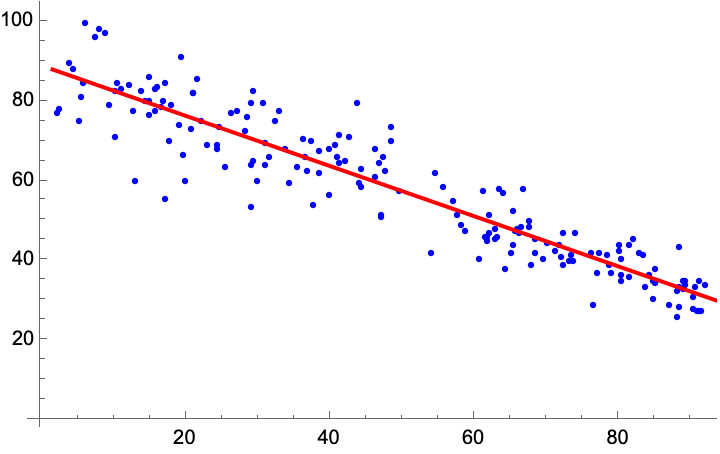
\includegraphics[width=0.45\textwidth]{xmas_spirit.png}
	\end{figure}

\begin{enumerate}[(a)]
\item Find $b_0$ and $b_1$ for this model. 
\item Was Christmas spirit positively or negatively correlated with age? Explain.
\item If a participant in this study, aged 29, rated their Christmas spirit as 62, find the residual for this individual. 
\item Find and interpret the coefficient of determination. 
\item Based on (d), is this a `good' linear model? Explain. 
\end{enumerate} 

\sol 
\begin{enumerate}[(a)]
\item We know that a linear model takes the form $\widehat{y}= b_1x + b_0$. We have $\widehat{y}= \widehat{S}$ and $x= a$. Therefore, we have $b_0= 87.98$ and $b_1= -0.62$. \pspace

\item Examining the plot of the linear model, we can see that Christmas spirit is negatively correlated with age. Alternatively, we can see that $b_1= -0.62 < 0$. Therefore, the variables are negatively correlated. Alternatively, we see that the (Pearson) correlation coefficient is negative, i.e. $r= -0.956971 < 0$. Therefore, the variables are negatively correlated. \pspace

\item We use our model to predict one's level of Christmas spirit at age 29. This is $\widehat{S}(a)$ when $a= 29$. We have $\widehat{S}(29)= 87.98 - 0.62(29)= 70$. But then the residual is $e= y - \widehat{y}= 62 - 70= -8$. \pspace

\item The coefficient of determination is $r^2$. This is $r^2= (-0.956971)^2= 0.915793494841$. Therefore, the data is `91.58\%' linear; that is, 91.58\% of the variation in Christmas spirit is linearly explained by one's age. \pspace

\item Yes, we have $r^2 \approx 0.9158 > 0.90$ (or $> 0.80$ or $> 0.60$) so that this is a good model. 
\end{enumerate}
	

\end{questions}
\end{document}